\bgroup
\begin{frame}{Gradient descent}
\begin{minipage}{0.6\textwidth}
\begin{itemize}
\item Let $J(\textbf{w})$ be a differentiable function of parameter vector $\textbf{w}$
\item Define the gradient of $J(\textbf{w})$ to be 
\begin{equation*}
\nabla_{\textbf{w}}J(\textbf{w})=\left(
                \begin{array}{c}
                  \frac{\delta J(\textbf{w})}{\delta \textbf{w}_1}\\
                  \vdots\\
                  \frac{\delta J(\textbf{w})}{\delta \textbf{w}_n}
                \end{array}
              \right)
\end{equation*}
\item To find a local minimum of $J(\textbf{w})$
\item Adjust $\textbf{w}$ in direction of -ve gradient
\begin{equation*}
\Delta \textbf{w} = -\frac{1}{2}\alpha\nabla_{\textbf{w}} J(\textbf{w})
\end{equation*}
where $\alpha$ is a step-size parameter
\end{itemize}
\end{minipage}
\begin{minipage}{0.35\textwidth}
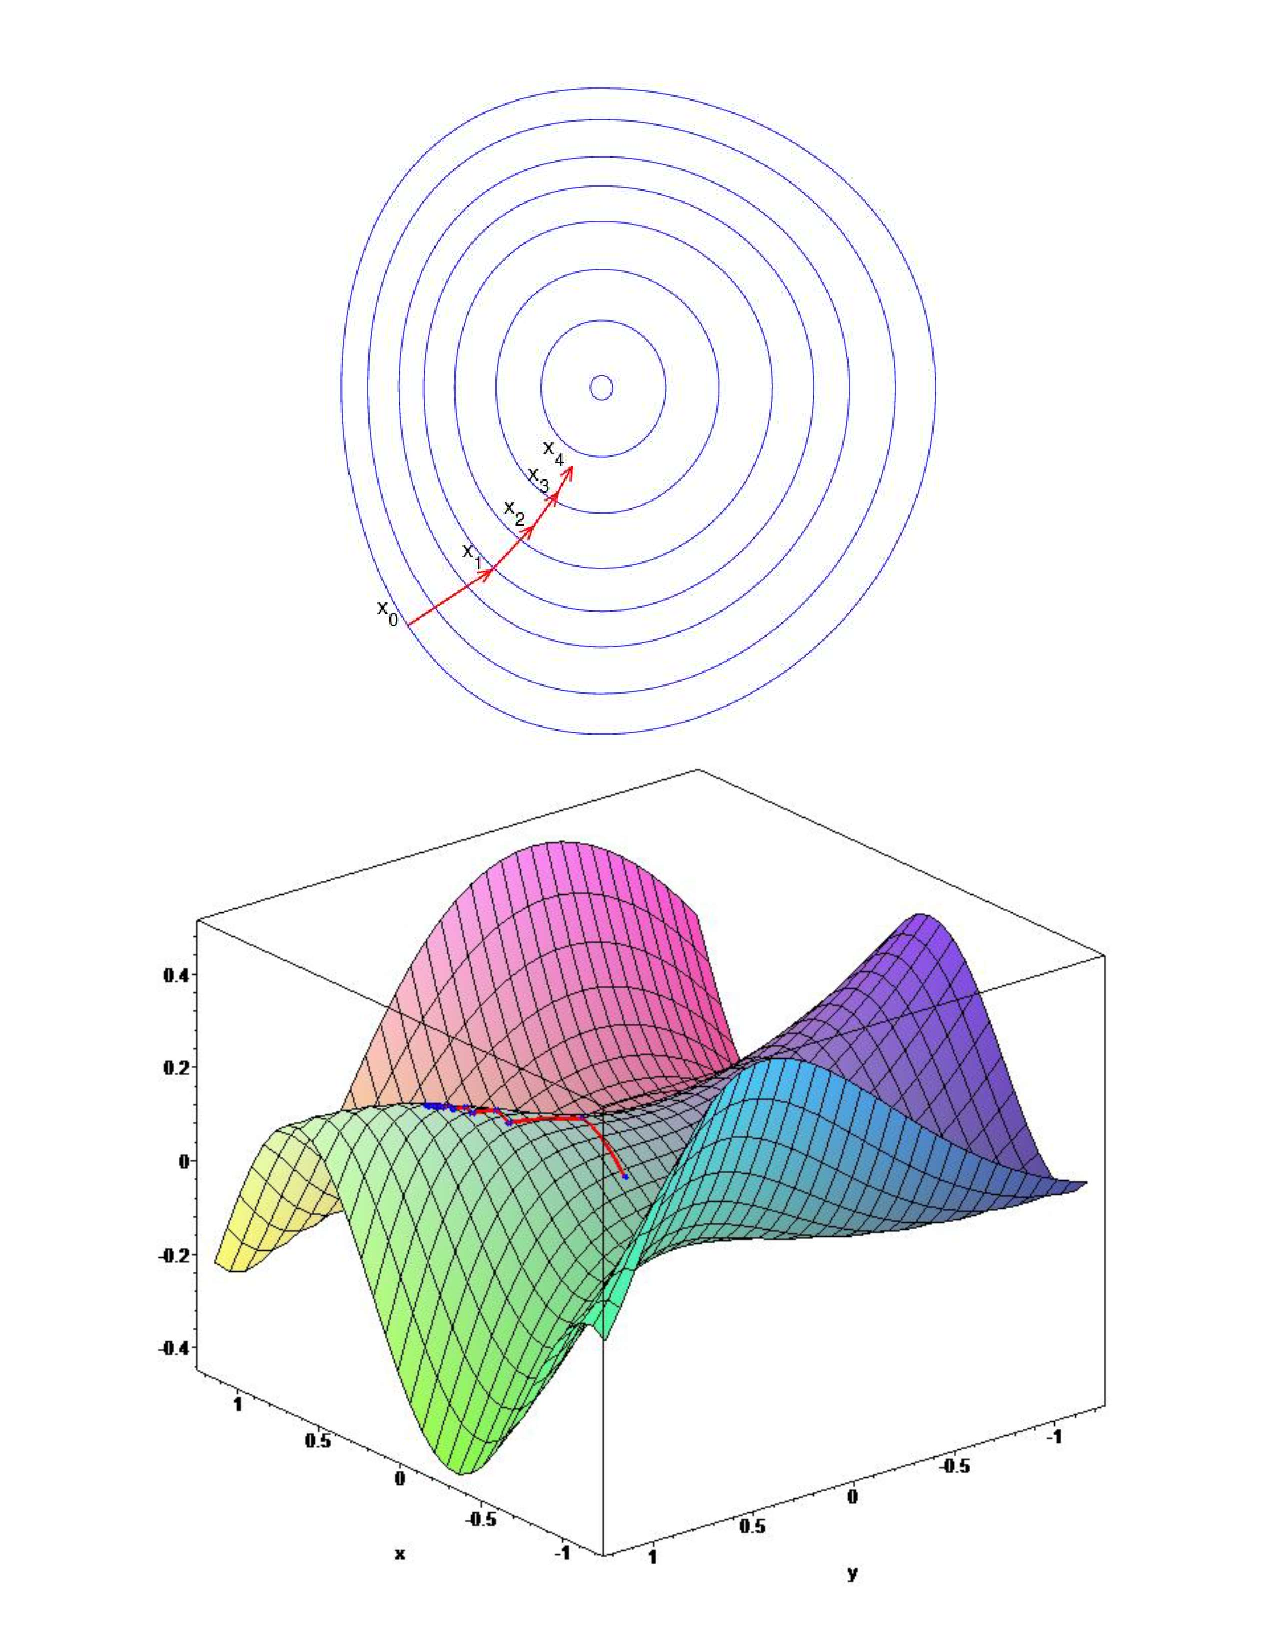
\includegraphics[width=\textwidth]{img/gd.pdf}
\end{minipage}
\end{frame}
\egroup